\documentclass[5pt]{article}
\usepackage{array}
\usepackage{listings}
\usepackage{graphicx}
\usepackage{color}
\usepackage{hyperref}
\usepackage{blindtext}
\usepackage[cache=false]{minted}

\definecolor{bg}{rgb}{0.95,0.95,0.95}
\title{Rapport M3102 TD/TP} 
\author{TUELEAU Tom}
\date{Janvier 2022}


\begin{document}
    \maketitle    
    \tableofcontents
    \newpage
    \section{Presentation}
    Pour la redaction de ce rapport je me suis servis des etapes donnees sur moodle afin de rediger ce document. Tout les sources utiliser seront citer tout au long du document. Tout le long des TP et TD j'ai stocker mon travail sur un repos github. Le lien est le suivant \url{https://github.com/Arakio34/tomtraceroute}.
    
    %Liste des rfc lue

    \section{Description des rfc}
    Lors de cette partie nous verrons les RFC que j'ai trouver pertinente pour d'écrire le fonctionnement des réseaux. En premier lieux les rfc que j'ai décider de vous presenter sont les suivante. 
    \begin{center}
        \begin{tabular}{|l|l|}
            \hline
            Numéros de rfc & Titre \\
            \hline
            rfc793 & TCP \\
            \hline
            rfc768 & UDP \\
            \hline
            rfc791 & IP \\
            \hline
            rfc3232 & Numéros de ports \\
            \hline
            rfc1918 & Réseaux privés \\
            \hline
        \end{tabular}
    \end{center}
    Dans un premier temps les rfc 793, 768 et 791 mon parus importante car décrivant trois des protocoles les plus utiliser. Les rfc 3232 et 1918 sont a mon sens important car elles permet de comprendre comment ce construit un réseaux ces liaisons.  
    %Liste des protcol
    \section{Definir les protocoles les plus utilises sur internet}
    Une fois les recherches effectuer sur les RFC faite, nous avions a lister les protocoles les plus utiliser d'internet. Les protocole regisent internet sont majoriterment definie par les rfc. Comme precedement voici la liste des protocoles que j'ai décider de citer :
     \begin{center}
        \begin{tabular}{|l|}
            \hline
            Protocoles \\
            \hline
            TCP \\
            \hline
            UDP \\
            \hline
             IP \\
            \hline
            OSPF \\
            \hline
            BGP \\
            \hline
        \end{tabular}
     \end{center}
    

    UDP et TCP sont deux protocoles de la couche transport qui permet la transmition de donnés. Ce sont eux qui font la base du transfer de donnés. Nous verrons plus tard que l'importance du protocole et du port utiliser pour effectuer la carte est important, certains routeur n'acceptant pas certains protocole. \\
         Il m'as paru aussi important de citer les deux protocole de routage que sont BGP et OSPF. BGP etants le protocole permetant de partager des routes entre AS et OSPF les routes entre routeur.  
    
    %Description de traceroute
    \section{Traceroute}
    Traceroute est un programme qui permet de tracer la route vers une URL/IP. Ce programme peut prendre plusieurs options, notament afin de preciser le protocole a utiliser pour tracer la route. Nous allons commencer par voire le fonctionement de traceroute en generale et ensuite de ces options.

         \subsection{Fonctionement}
         Le principe du fonctionement est asser simple. Il conciste a l'envoie de paquets touts en augmentant a chaque fois de 1 le TTL. Cela permet donc de recevoir une reponse de tout les routeur parcouru. Parmis les option on peut directement modifier le TTL maximum (30 de base) avec l'option -m.
      
        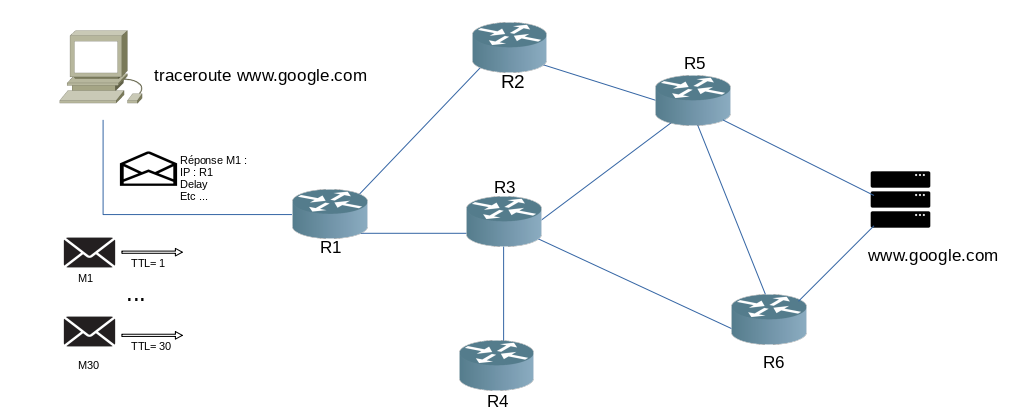
\includegraphics[scale=0.5]{1.png} 

      
      Exemple :
      \begin{minted}[breaklines]{bash}
        tueleau-tom [172.42.70.101/24] ~ $ sudo traceroute google.com
        traceroute to google.com (142.251.37.206), 30 hops max, 60 byte packets
        1  _gateway (172.42.70.254)  0.313 ms  0.248 ms  0.213 ms
        2  gw.iutbeziers.fr (194.199.227.254)  0.841 ms  0.804 ms  0.770 ms
        3  100.75.85.254 (100.75.85.254)  6.058 ms  6.074 ms  6.043 ms
        4  100.75.1.6 (100.75.1.6)  8.918 ms  8.888 ms  8.915 ms
        5  10.3.4.1 (10.3.4.1)  6.753 ms  6.797 ms  6.760 ms
        6  193.55.200.138 (193.55.200.138)  6.346 ms  6.342 ms  6.295 ms
        7  xe-1-0-12-ren-nr-marseille1-rtr-131.noc.renater.fr (193.51.180.191)  13.657 ms xe-1-0-16-marseille1-rtr-131.noc.renater.fr (193.51.177.18)  13.096 ms  13.041 ms
        8  xe-0-0-15-marseille2-rtr-131.noc.renater.fr (193.51.180.116)  8.424 ms xe-1-0-10-marseille2-rtr-131.noc.renater.fr (193.51.180.120)  9.238 ms xe-1-0-6-marseille2-rtr-131.noc.renater.fr (193.51.177.213)  9.229 ms
        9  72.14.218.132 (72.14.218.132)  15.236 ms  8.579 ms  8.571 ms
        10  74.125.244.225 (74.125.244.225)  9.533 ms  9.526 ms  9.533 ms
        11  142.251.78.83 (142.251.78.83)  8.533 ms  8.524 ms  8.499 ms
        12  mrs09s15-in-f14.1e100.net (142.251.37.206)  8.533 ms  8.486 ms  8.515 ms
        tueleau-tom [172.42.70.101/24] ~ $ sudo traceroute -m 4 google.com
        traceroute to google.com (142.251.37.206), 4 hops max, 60 byte packets
        1  _gateway (172.42.70.254)  0.223 ms  0.212 ms  0.266 ms
        2  gw.iutbeziers.fr (194.199.227.254)  0.811 ms  0.804 ms  0.798 ms
        3  100.75.85.254 (100.75.85.254)  6.671 ms  6.665 ms  6.658 ms
        4  100.75.1.6 (100.75.1.6)  7.433 ms  7.673 ms  7.666 ms

      \end{minted}
      Comme nous pouvons le voire ci-dessus une fois l'option "-m 4" rajouter le traceroute s'arret aux 4 éme routeur.
      
      \subsection{Option}
       J'ai eux donc l'occasion d'utiliser de multiple option afin de tester le packet. Comme vue precedement nous avons le -m permétent de réduire le TTL max.  Ci-dessous la liste des option utiliser avec une description de ce qu'elle font.

       \begin{center}
        \begin{tabular}{|l|l|}
            \hline
            Option & Description \\
            \hline
             -m & Permet de specifier la valeur maximum du TTL (30 de base). \\
            \hline
            -U &  Permet de choisir le protocole UDP pour l'émission des paquets. \\
            \hline
            -T &  Permet de choisir le protocole TCP pour l'émission des paquets. \\
            \hline
            -I &  Permet de choisir le protocole ICMP  pour l'émission des paquets. \\
            \hline
            -i & Permet de choisir l'interface que l'on souhaite utiliser. \\
            \hline
            -f & Définie la taille du TTL du permier paquet envoyer. \\
            \hline
            -\-port & Permet de donner le port a cibler lors de l'envoie des paquets. \\
            \hline
        \end{tabular}
    \end{center}
    L'interet des option permetant de changer le protocole est que certains routeur ne reponde que sur certain ports / protocole. Cela permet donc d'obtenir les routes les plus précises.

    %Description du script creer
    \section{Script}
    Le script que j'ai creer permet plusieurs chose. Tout d'abords il permet de tracer les routes en fonction des URL donner et des protocoles. Cella permet donc de voire qu'elles routeurs acceptes ou non certains protocoles. Il y a differents moyen de l'utiliser mais pour cella je vous laisse lire la page d'aide. Je vais plutôt décrire le fonctionnement du traitement des données. 


    \subsection{Recupération et }

    \begin{minted}[breaklines,bgcolor=bg]{bash}
    protocole=("-I") # "-U" "-T" "-T-p80" "-T-p22" "-T-p20")
	declare -A shapePRO=( ['-U']="normal" ['-I']="diamond" ['-T']="vee" ['-D']="crow" ['-T-p80']="tee" ['-T-p22']="box" ['-T-p20']="dot" )
	color=( "red" "blue" "purple" "green" "brown" "coral" "darkorange" "gray" "gold" "pink" "cyan" "silver" "tomato" "slateblue" "webmaroon" "skyblue")
	echo > dote.dot
	urlia=\$@
            
    # Debut de la carte 
    echo "digraph A {" >>dote.dot

    # Creation de la legende. 
    for pro in \${protocole[@]}
	do
		shape=\${shapePRO[\$pro]}
		echo "\"PROTOCOLE\"->\"prot = \$pro\"->\"\$shape\"[arrowhead=\$shape]" >> dote.dot
	done
    
    y=0
	for url in \${urlia[@]}
	do
		echo " \"URL\" -> \"url = \$url\"->\"\${color[\$y]}\"[color=\${color[\$y]}]" >> dote.dot
		y=\$y+1
	done

    # Debuts de la route.
    i=0
	for url in \${urlia[@]}
	do	
		echo -e "Traceroute sur \e[31m\$url \e[39m..."
		for pro in \${protocole[@]}
		do
			echo "\$pro"
			echo > \$url\$pro 
			prob=\$(echo \$pro | sed "s/\-/ \-/g") 
			traceroute -A \$prob \$url >> \$url\$pro
			sed -i '2d' \$url\$pro                
			cat \$url\$pro | grep -o -E "(\([[:digit:]]{1,3}\.[[:digit:]]{1,3}\.[[:digit:]]{1,3}.[[:digit:]]{1,3})|(AS[[:digit:]]{1,})|(\* \* \*)" > p\$url\$pro 
			rm \$url\$pro
			element=\$(cat p\$url\$pro |sed "s/(/ /g"|sed -r -e':a;N;\$!ba;s/((\* \* \*\n))//g'| sed ':a;N;\$!ba;s/\nA/ A/g' | sed ':a;N;\$!ba;s/\n/\"\-\>\"/g')
			shape=\${shapePRO[\$pro]}
			bienfini=\$(tail -n1 p\$url\$pro)
			if [ "\$bienfini" = "* * *" ]
			then
				echo "\"\$element\"[arrowhead=\$shape, color=\${color[\$i]}]" >> dote.dot 
			else
				echo "\"\$element\"->\"\$url\"[arrowhead=\$shape, color=\${color[\$i]}]" >> dote.dot
			fi
			rm p\$url\$pro
		done
		i=\$i+1
	done

	#Fin du digraph
	echo "}" >> dote.dot
    mv dote.dot dote1.dot
    
    #On retire les bulles vides.	
    cat dote1.dot | sed -r "s/(\"\"\->(.){1,})//g" > dote.dot
	dot -Tpng dote.dot > dote.png
	rm dote1.dot
	exit

\end{minted}


    %Annalyse des anomalies trouver
    \section{Anomalies}


\end{document} 



function Trsolo () {

function Trfichier () {
	file=$1
	a=$(cat $file)
	urlfichier=$(echo $a)
	Trsolo $urlfichier
	exit
}

function Predef () {
    tab_URL=("www.umontpellier.fr" "www.iutbeziers.fr" "www.google.com" "ac-versailles.fr" "ac-montpellier.fr" "www.idf.iut.fr" "8.8.8.8" "1.1.1.1" "cisco.fr" "cisco.com" "stormshield.eu" "www.ac-paris.fr" "ac-toulouse.fr" "ac-lyon.fr" "ac-clermont.fr" "ac-bordeaux.fr")
    Trsolo ${tab_URL[@]}
}


while getopts "ahu:f:" option; do
    case "$option" in
        h) # Affiche l'aide.
            echo "Page d'aide."
            Help
            exit
            ;;
    	f) # Utilise un fichier pour les URL/IP.
            echo "Mode fichier." 
	        fileurl=$OPTARG
	        Trfichier $fileurl
	        exit
            ;;
        u) # Permet de donnes une URL/IP en arguments.
            echo "Mode solo URL." 
            url=$OPTARG
            Trsolo $url
            exit
            ;;
        a) # Utilise les URL et IP predefinie.
            echo "Mode predefinie." 
            Predef
    	    exit
            ;;
        *)
            Help
            exit
            ;;
    esac
done
Help
